\documentclass{article}
\usepackage{tikz}

\begin{document}

\begin{figure}[htbp]
    \centering
    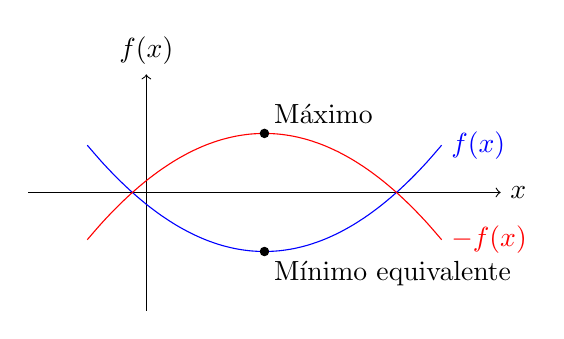
\begin{tikzpicture}[scale=1.5]
        % Eixo x
        \draw[->] (-1,0) -- (3,0) node[right] {$x$};
        % Eixo y
        \draw[->] (0,-1) -- (0,1) node[above] {$f(x)$};
        % Função f(x)
        \draw[domain=-0.5:2.5,smooth,variable=\x,blue] plot ({\x},{0.4*(\x-1)^2 - 0.5}) node[right] {$f(x)$};
        % Função -f(x)
        \draw[domain=-0.5:2.5,smooth,variable=\x,red] plot ({\x},{-0.4*(\x-1)^2 + 0.5}) node[right] {$-f(x)$};
        % Ponto máximo
        \filldraw[black] (1,0.5) circle (1pt) node[above right] {Máximo};
        % Ponto mínimo equivalente
        \filldraw[black] (1,-0.5) circle (1pt) node[below right] {Mínimo equivalente};
    \end{tikzpicture}
    \caption{Maximizar $f(x)$ é equivalente a minimizar $-f(x)$.}
    \label{fig:max_min_equiv}
\end{figure}

\end{document}
